\newcommand{\TRESicmin}{1.85\xspace}
\newcommand{\TRESicmax}{3.10\xspace}
\newcommand{\TRESicNoveNoveMin}{1.62\xspace}
\newcommand{\TRESicNoveNoveMax}{3.33\xspace}
\newcommand{\TRESnZero}{26\xspace}


\subsection{Teste de Hipótese}

	Para testar a hipótese de que a renda média mensal dos alunos é menor
	que $4,5$ salários mínimos, deve ser aplicado um teste de hipótese com a
	média. Nesse caso, a hipótese nula ($H_0$) é de que a remédia média mensal dos
	alunos é superior ou igual a $4,5$ salários mínimos e a hipótese alternativa
	($H_1$) é de que a renda média mensal dos alunos é inferior a $4,5$ salários
	mínimos. O nível de significância para o teste é de $5\%$.
	%
	\begin{align*}
		H_0: \mu &= 4,5\\
		H_1: \mu &< 4,5   \\
		     \alpha &= 0,05
	\end{align*}

	Como o desvio padrão da população é desconhecido, a estatística do
	teste é expressa pelo valor $t$ da Distribuição $t$ de Student, com grau de
	liberdade $\DOISgrauLiberdade$:
	%
	\begin{align*}
		t_{19} &= \frac{(\bar{x} - \mu_0)\cdot\sqrt{n}}{s} \\
		t_{19} &= \dfrac{(\DOISmediaAmostra - \DOISmediaPopulacao) \cdot \sqrt{\DOIStamanhoAmostra}}{\DOISdesvioAmostra} \\
		t_{19} &= \DOISteste
	\end{align*}

	Com o auxílio do software estatístico R, calculou-se $P(t  \leq t_{19})
	= -4.83\times 10^{-10}$ através da função \texttt{pt()}. Como $P(t  \leq
	t_{19}) < \alpha$ rejeita-se a hipótese nula. Ou seja, há evidências
	estatísticas de que a média mensal dos alunos é menor que $4,5$ salários
	mínimos com $5\%$ de nível de significância.

\subsection{Poder do Teste}

	Para calcular o poder do deste, deve-se empregar a distribuição não
	central $t$ de Student. Portanto, deve-se, primeiramente, calcular o fator de
	não centralidade em salários mínimos.
	%
	\begin{align*}
		d_{3,50} &= -\DOISabicissaA\\
		d_{3,75} &= -\DOISabicissaB\\
		d_{3,85} &= -\DOISabicissaC\\
		d_{3,95} &= -\DOISabicissaD\\
		d_{4,15} &= -\DOISabicissaE\\
		d_{4,25} &= -\DOISabicissaF\\
		d_{4,35} &= -\DOISabicissaG\\
	\end{align*}

	Com posse desses dados o poder desses valores, o poder do teste
    pode ser calculado com a função \texttt{pwr.t.test()} do software
    estatístico R. Para o teste, considerou-se o nível de
    significância $1\%$ e o desvio padrão amostral como estimativa do
    desvio padrão populacional (como $d_\mu$ é expresso em salários
    mínimos, o desvio padrão é fornecido para
    \texttt{pwr.t.test}). Para cada valor de $\mu$, o poder do teste é
    mostrado a seguir:
	%
	\begin{align*}
		1 - \beta_{3,50} &= \DOISpoderA\\
		1 - \beta_{3,75} &= \DOISpoderB\\
		1 - \beta_{3,85} &= \DOISpoderC\\
		1 - \beta_{3,95} &= \DOISpoderD\\
		1 - \beta_{4,15} &= \DOISpoderE\\
		1 - \beta_{4,25} &= \DOISpoderF\\
		1 - \beta_{4,35} &= \DOISpoderG\\
	\end{align*}

\subsection{Análise do Poder de Teste}

	A análise do poder de teste com amostras de tamanho $40$, $50$, $60$ e $70$
	é apresentada na \autoref{figure: poder do teste renda}. Em todos os casos o
	nível de significância foi fixado em $1\%$ e o desvio padrão amostral fixado
	em $\DOISdesvioAmostra$, o desvio padrão amostral obtido com amostra de
	tamanho 20.

	Analisando o gráfico é possível constatar que, quanto maior o tamanho da
	amostra, maior o poder do teste, e quanto mais próxima a média populacional
	é daquela fixada na hipótese nula (4.5), menor o poder do teste. A escolha correta
	do tamanho da amostra depende de de dois fatores: (a) facilidade para
	obtenção de amostras; e (b) poder do teste desejado.
	
	Considerando esses dois fatores como de igual importância, a
    \autoref{figure: poder do teste e tamanho da amostra renda} resume
    essa relação em um único fator $\dfrac{\text{poder do
        teste}}{\text{tamanho da amostra}}$. Por análise, para a detecção de
    médias reais inferiores a $3.9$ salários, uma amostra de $40$ é
    a mais indicada, pois esta apresenta retorno por elemento da
    amostra maior que todos os demais tamanhos de amostra.  no entanto,
    quando a média real é maior que $3.9$, e portanto mais próxima da
    média usada em $H_0$, todos os tamanhos de amostra apresentam
    proporções de retorno por elemento de amostra similares. Portanto,
    nesse caso o tamanho de amostra a ser escolhido é $70$, pois este
    proverá maior poder ao teste.


	\begin{figure}[!h]
		\centering
		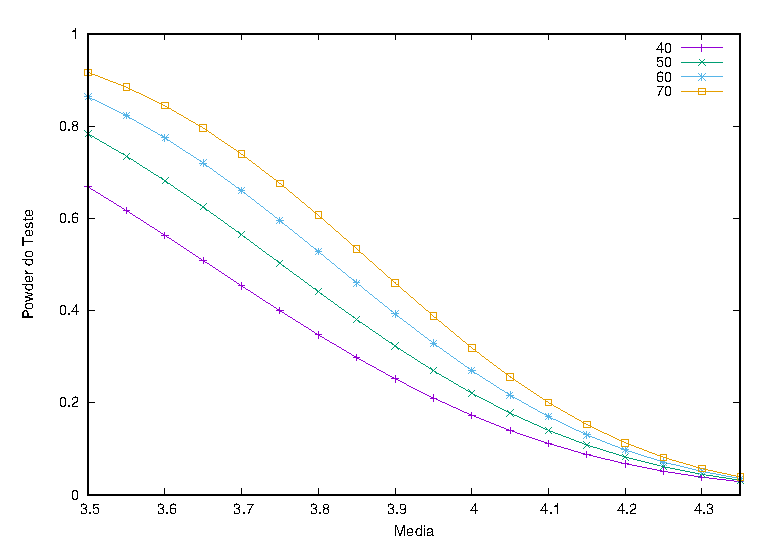
\includegraphics[width=0.8\linewidth]{questao2/powers.eps}
		\caption{Curva característica de operação para variável \textit{Renda}}
		\label{figure: poder do teste renda}
	\end{figure}

	\begin{figure}[!h]
		\centering
		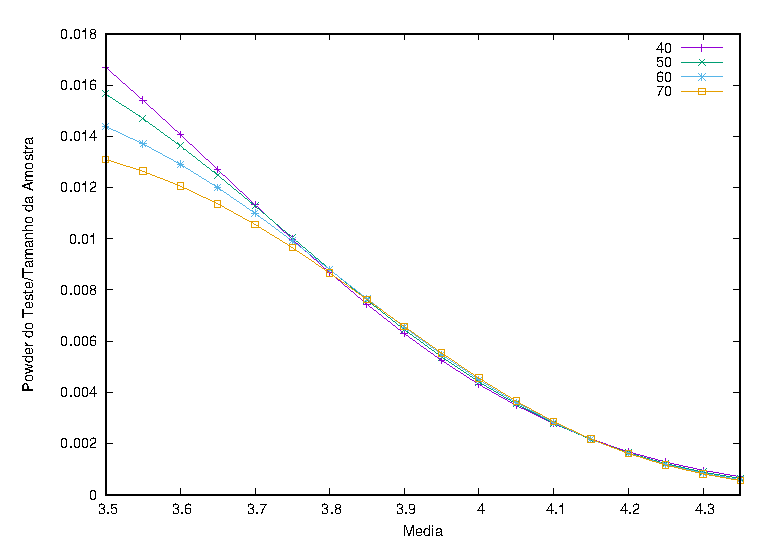
\includegraphics[width=0.8\linewidth]{questao2/powers-breakdown.eps}
		\caption{Poder do teste em relação ao tamanho da amostra para a variável \textit{Renda}}
		\label{figure: poder do teste e tamanho da amostra renda}
	\end{figure}

\subsection{Tamanho da Amostra}

	Para calcular o tamanho mínimo da amostra para detectar com $95\%$ de
	probabilidade que a média de renda dos alunos é de 4 salários mínimos,
	deve-se utilizar um teste baseado na distribuição não central $t$ de Student.
	Para tanto, foi considerada a amostra piloto de 20 observações, $1\%$ de
	nível de significância e o desvio padrão amostral como uma boa estimativa do
	desvio padrão populacional. O cálculo foi efetuado usando o seguinte
	fragmento do software R.

	Com esse análise contastou-se que para detectar essa característica, uma
	amostra de no mínimo 34 observações se faz necessária. Portanto, a amostra
	retirada de tamanho 20 é insuficiente para evidenciar essas conclusões.

%%% Local Variables:
%%% mode: latex
%%% TeX-master: "../main"
%%% End:
